%% ============================================================
%%  Informe Proyecto Final - IA - EAFIT 2026-1
%%  MatchMind: Prediccion de Resultados de Futbol Internacional
%%  Integrantes: Matias Martinez Moreno, Samuel Herrera
%% ============================================================

\documentclass[10pt,twocolumn]{article}

\usepackage[utf8]{inputenc}
\usepackage[T1]{fontenc}
\usepackage[spanish]{babel}
\usepackage[margin=1.8cm, top=2.2cm, bottom=2.2cm]{geometry}
\usepackage{lmodern}
\usepackage{microtype}
\usepackage{palatino}

\usepackage{amsmath, amssymb}
\usepackage{graphicx}
\usepackage[dvipsnames,svgnames]{xcolor}
\usepackage{booktabs}
\usepackage{tabularx}
\usepackage{multirow}
\usepackage{array}
\usepackage{listings}
\usepackage{hyperref}
\usepackage{enumitem}
\usepackage{float}
\usepackage{caption}
\usepackage{subcaption}
\usepackage{fancyhdr}
\usepackage{titlesec}

\definecolor{eafitblue}{RGB}{0, 61, 121}
\definecolor{eafitgreen}{RGB}{0, 150, 80}
\definecolor{eafitgray}{RGB}{90, 90, 90}
\definecolor{codebg}{RGB}{248, 248, 252}
\definecolor{codecomment}{RGB}{100, 110, 130}
\definecolor{codekw}{RGB}{0, 90, 170}
\definecolor{codestr}{RGB}{160, 50, 0}

\lstset{
  backgroundcolor=\color{codebg},
  basicstyle=\ttfamily\scriptsize,
  keywordstyle=\color{codekw}\bfseries,
  commentstyle=\color{codecomment}\itshape,
  stringstyle=\color{codestr},
  numbers=left,
  numberstyle=\tiny\color{eafitgray},
  numbersep=6pt,
  frame=single,
  framesep=3pt,
  rulecolor=\color{eafitblue!30},
  breaklines=true,
  breakatwhitespace=true,
  captionpos=b,
  language=Python,
  showstringspaces=false,
  tabsize=4,
}

\titleformat{\section}
  {\normalfont\bfseries\large\color{eafitblue}}
  {\thesection.}{0.6em}{}
  [\vspace{-2pt}\color{eafitblue!35}\hrule\vspace{4pt}]

\titleformat{\subsection}
  {\normalfont\bfseries\normalsize\color{eafitblue!80}}
  {\thesubsection.}{0.5em}{}

\pagestyle{fancy}
\fancyhf{}
\fancyhead[L]{\small\color{eafitgray}\textit{MatchMind - Proyecto Final IA - EAFIT 2026-1}}
\fancyhead[R]{\small\color{eafitgray}\thepage}
\fancyfoot[C]{\small\color{eafitgray!60}Matias Martinez Moreno y Samuel Herrera}
\renewcommand{\headrulewidth}{0.4pt}

\hypersetup{
  colorlinks=true,
  linkcolor=eafitblue,
  citecolor=eafitgreen,
  urlcolor=eafitblue!80,
  pdftitle={MatchMind - Proyecto Final IA EAFIT 2026},
  pdfauthor={Matias Martinez, Samuel Herrera},
}

\captionsetup{font=small, labelfont={bf,color=eafitblue}, skip=4pt}

\newcommand{\nota}[1]{%
  \vspace{4pt}
  \noindent\colorbox{eafitblue!8}{%
    \begin{minipage}{\columnwidth-2\fboxsep}
      \small\color{eafitblue!80}\textbf{Nota:} #1
    \end{minipage}
  }
  \vspace{4pt}
}

\begin{document}

%% =====================  PORTADA  =====================
\twocolumn[{%
\begin{center}
  {\color{eafitblue!25}\rule{\linewidth}{3pt}}\\[6pt]
  {\Large\bfseries\color{eafitblue}
    MatchMind: Prediccion de Resultados de Partidos Internacionales de Futbol\\[4pt]
  }
  {\normalsize\color{eafitgray}
    XGBoost con explicabilidad SHAP y analisis tactico generado por LLM\\[10pt]
  }

  \begin{tabular}{cc}
    \textbf{Matias Martinez Moreno} & \textbf{Samuel Herrera} \\
    \small ID: 1000117104 & \small ID: 1000358613 \\
    \small Grupo: Jueves & \small Grupo: Jueves
  \end{tabular}\\[10pt]

  {\small\color{eafitgray}
    Escuela de Ciencias Aplicadas e Ingenieria - Universidad EAFIT\\
    Curso: Inteligencia Artificial - Semestre 2026-1\\
    \textit{Entrega: 14 de mayo de 2026}\\[4pt]
    \textbf{Repositorio:}
    \url{https://github.com/matias-martinez-moreno/matchmind-ia-eafit}
  }\\[6pt]
  {\color{eafitblue!25}\rule{\linewidth}{1pt}}\\[10pt]
\end{center}
}]

%% =====================  ABSTRACT  =====================
\begin{abstract}
\noindent
\textbf{Contexto.} La prediccion de resultados de partidos de futbol es un problema clasico de clasificacion multiclase que combina alta varianza estocastica (los resultados son inciertos por naturaleza) con senales sistemicas predecibles (ranking, ventaja de localia, historial entre rivales). Es un caso de estudio ideal porque tiene datos abundantes, etiquetas claras y un techo teorico bajo: incluso los mejores modelos publicados rara vez superan accuracy de 0.60.
\textbf{Objetivo.} Construir un sistema completo que: (1) prediga el resultado de un partido internacional entre tres clases (victoria local, empate, victoria visitante), (2) explique la prediccion con valores SHAP, y (3) genere un analisis tactico narrativo en espanol mediante un LLM.
\textbf{Metodo.} XGBoost entrenado sobre 30,511 partidos posteriores a 1993, con 14 features ingenierizadas (rachas recientes de victorias, promedios moviles de goles, head-to-head historico, ranking FIFA, neutralidad del campo). Explicabilidad con SHAP TreeExplainer. Un LLM (Llama-3.1-8b vía Groq API) recibe los top-5 features SHAP como contexto para producir el reporte narrativo.
\textbf{Resultados.} F1-macro = 0.452 en test (5,876 partidos 2020-2026), accuracy = 0.549, AUC-OvR = 0.707, frente a un baseline trivial de F1-macro = 0.215. El LLM cumple el 100\% del criterio de mencionar factores SHAP relevantes y respetar el limite de palabras.
\textbf{Conclusion.} El sistema duplica el F1-macro del baseline. Queda documentado como limitacion principal que el modelo subpredice los empates, fenomeno conocido en la literatura del area.\\[4pt]

\textbf{Palabras clave:} XGBoost, SHAP, LLM, Llama-3.1, prediccion de futbol, clasificacion multiclase, ranking FIFA.
\end{abstract}

\vspace{4pt}

%% ==========================================================
\section{Introduccion}
%% ==========================================================

Predecir el resultado de un partido de futbol parece imposible: por algo lo llaman ``el deporte mas hermoso del mundo''. Sin embargo, cuando uno analiza miles de partidos en lugar de uno solo, aparecen patrones claros. Equipos con mejor ranking ganan mas seguido, los locales aprovechan su cancha y los rivales tradicionales producen resultados ajustados con frecuencia. Estos patrones son lo que un modelo de Machine Learning puede capturar: no para acertarle a cada partido, sino para asignar probabilidades realistas.

En este trabajo construimos \textbf{MatchMind}, un sistema end-to-end con tres componentes integrados: (a) un clasificador XGBoost que estima la probabilidad de cada uno de los tres resultados posibles, (b) una capa de explicabilidad con SHAP que identifica que features influyeron mas en cada prediccion individual, y (c) un Large Language Model que toma esas explicaciones tecnicas y las traduce a un analisis narrativo comprensible para un aficionado.

La pregunta de investigacion que motiva el trabajo es:

\begin{quote}
  \textit{``Puede un modelo XGBoost predecir el resultado de partidos internacionales con F1-macro superior a 0.40, y puede un LLM generar analisis tacticos comprensibles usando los valores SHAP como contexto?''}
\end{quote}

El umbral de 0.40 no es arbitrario: un clasificador que siempre prediga la clase mayoritaria (``local gana'') obtendria F1-macro de apenas 0.215, asi que superar 0.40 ya implica que el modelo aprende patrones reales mas alla del balance de clases.

Usamos dos datasets publicos: \textit{International Football Results 1872-2024} (Kaggle), que contiene 49,287 partidos internacionales con goles, fecha, torneo y campo neutral o no \cite{kaggle_results}; y \textit{FIFA World Rankings} (Kaggle), con 67,472 filas del ranking FIFA historico desde 1992 \cite{kaggle_fifa}. Filtramos a partidos posteriores a 1993 para tener ranking confiable y eliminamos 72 partidos sin score (0.15\%), quedando 30,511 partidos utiles.

El resto del documento organiza el analisis exploratorio (Seccion 2), la arquitectura del sistema (Seccion 3), la metodologia y validacion (Seccion 4), los resultados cuantitativos (Seccion 5), la discusion de limitaciones (Seccion 6) y las conclusiones (Seccion 7).

%% ==========================================================
\section{Datos y Exploracion (EDA)}
\label{sec:eda}
%% ==========================================================

\subsection{Descripcion del dataset}

\begin{table}[H]
\centering
\caption{Resumen del dataset principal tras limpieza.}
\label{tab:dataset}
\begin{tabularx}{\columnwidth}{lX}
\toprule
\textbf{Atributo} & \textbf{Descripcion} \\
\midrule
Fuente & Kaggle (martj42 + cashncarry) \\
Registros crudos & 49,287 partidos \\
Filtro aplicado & post-1993 y sin nulos \\
Registros finales & 30,511 partidos \\
Features finales & 14 numericas \\
Variable objetivo & 3 clases (away/draw/home) \\
Periodo & 1993-2026 \\
\bottomrule
\end{tabularx}
\end{table}

\subsection{Hallazgo 1: imbalance moderado del target}

\begin{figure}[H]
  \centering
  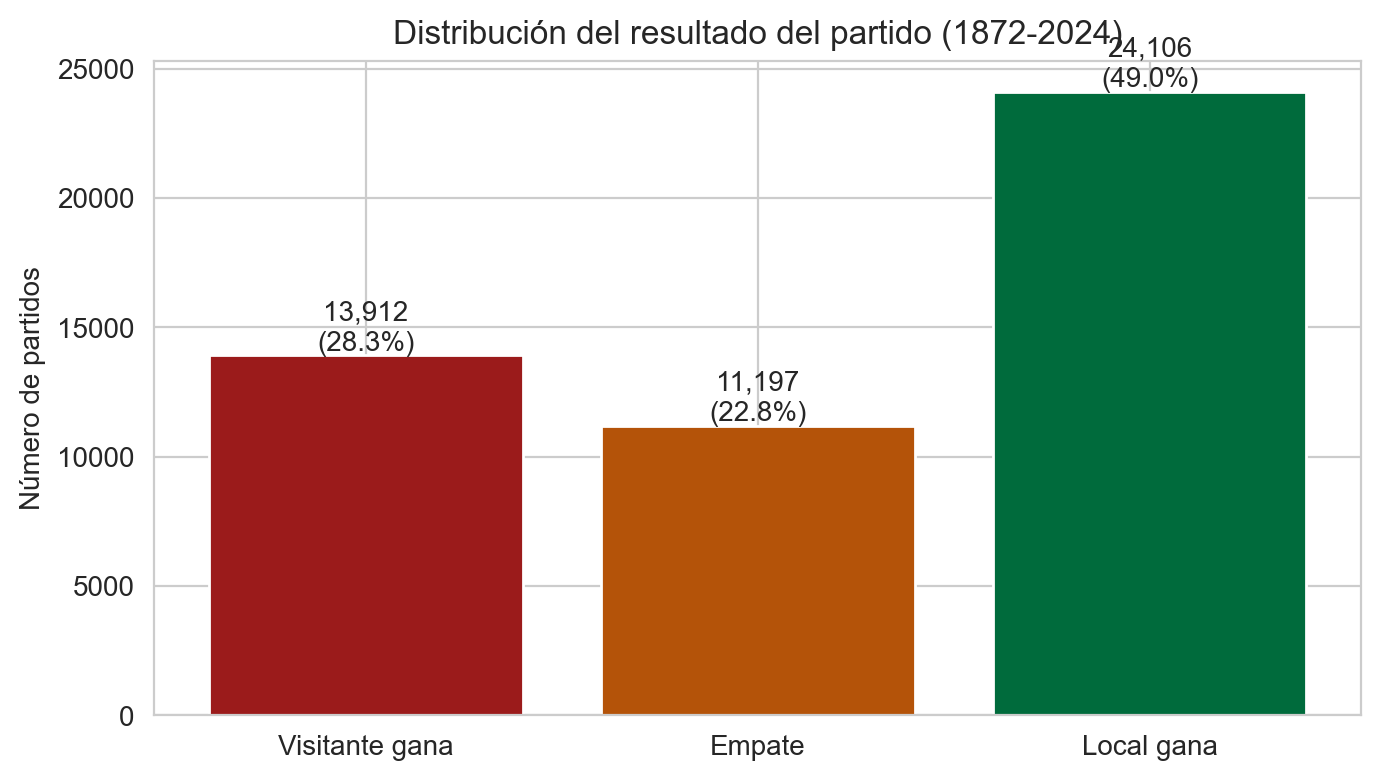
\includegraphics[width=\columnwidth]{figures/eda_distribucion.png}
  \caption{Distribucion del resultado del partido: 48.9\% victorias locales, 22.7\% empates, 28.4\% victorias visitantes. Calculado sobre 49,215 partidos historicos limpios.}
  \label{fig:eda_dist}
\end{figure}

La Figura~\ref{fig:eda_dist} muestra la distribucion del target. La clase mayoritaria (victoria local) representa el 48.9\% de los partidos. Este imbalance moderado tiene una consecuencia metodologica directa: \textbf{no podemos usar accuracy como metrica principal}. Un modelo trivial que prediga siempre ``local gana'' tendria 47.4\% de accuracy en test, lo cual suena decente pero es engañoso porque significa que el modelo solo memorizo la clase mas frecuente. Por eso reportamos \textbf{F1-macro}, que promedia el F1 de cada clase por igual, penalizando a modelos que ignoren las clases minoritarias. Ese mismo modelo trivial tiene F1-macro de apenas 0.215.

\subsection{Hallazgo 2: ventaja de localia cuantificada}

\begin{figure}[H]
  \centering
  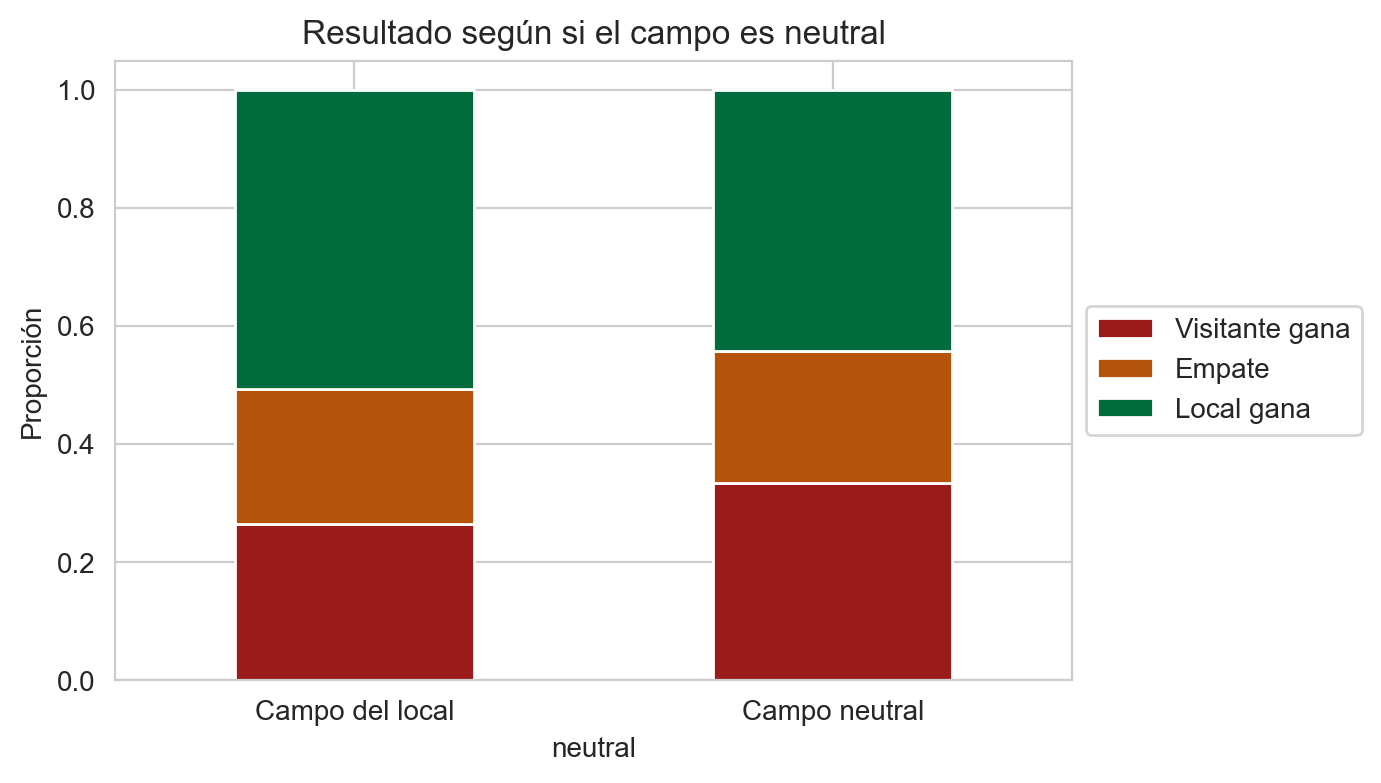
\includegraphics[width=\columnwidth]{figures/eda_localia.png}
  \caption{Distribucion del resultado segun si el campo es neutral o del equipo local. La ventaja de jugar en casa se traduce en +6.8 puntos porcentuales de victoria.}
  \label{fig:eda_localia}
\end{figure}

La Figura~\ref{fig:eda_localia} cuantifica un fenomeno bien conocido en el deporte: jugar en casa aumenta la probabilidad de ganar. Concretamente, el equipo local gana el 50.7\% de las veces cuando el partido se disputa en su pais, pero solo el 43.9\% cuando se juega en cancha neutral. La diferencia de 6.8 puntos porcentuales puede parecer pequena, pero acumulada sobre miles de partidos representa una senal estadisticamente fuerte. Esto justifica incluir la variable booleana \texttt{neutral} como feature del modelo.

\subsection{Hallazgo 3: el ranking FIFA es la senal mas predictiva}

\begin{figure}[H]
  \centering
  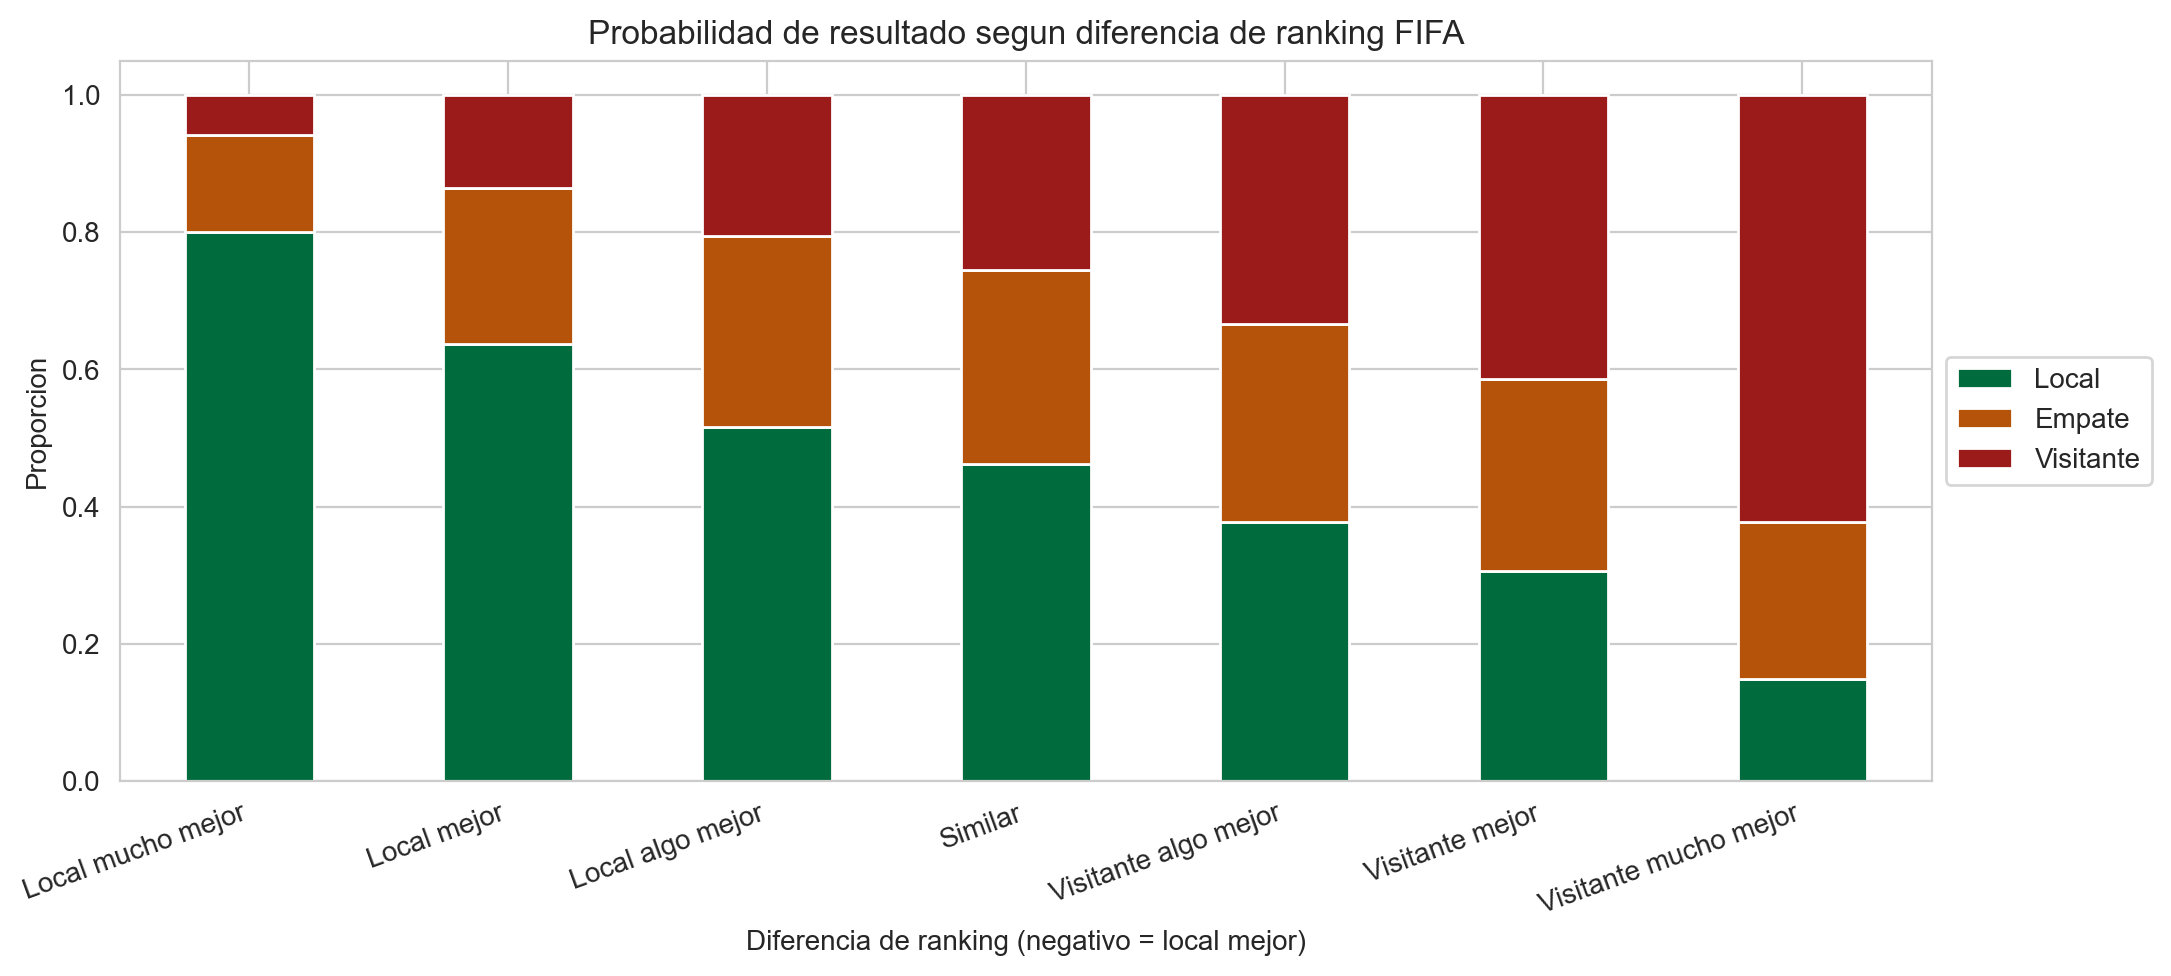
\includegraphics[width=\columnwidth]{figures/eda_ranking_resultado.png}
  \caption{Probabilidad de resultado segun la diferencia de ranking FIFA. Cuando el local es ``mucho mejor'' en el ranking, gana el 80\% de las veces; en el extremo opuesto, gana el visitante el 62\%.}
  \label{fig:eda_rank}
\end{figure}

La Figura~\ref{fig:eda_rank} es quiza la mas importante del analisis. Discretizamos la diferencia de ranking en siete tramos y graficamos la probabilidad de cada resultado en cada tramo. El patron es muy claro: a mayor ventaja en el ranking, mayor probabilidad de victoria. Esto confirma que el ranking FIFA, aunque imperfecto, captura informacion real sobre la calidad relativa de los equipos.

\subsection{Hallazgo 4: heatmap de correlaciones}

\begin{figure}[H]
  \centering
  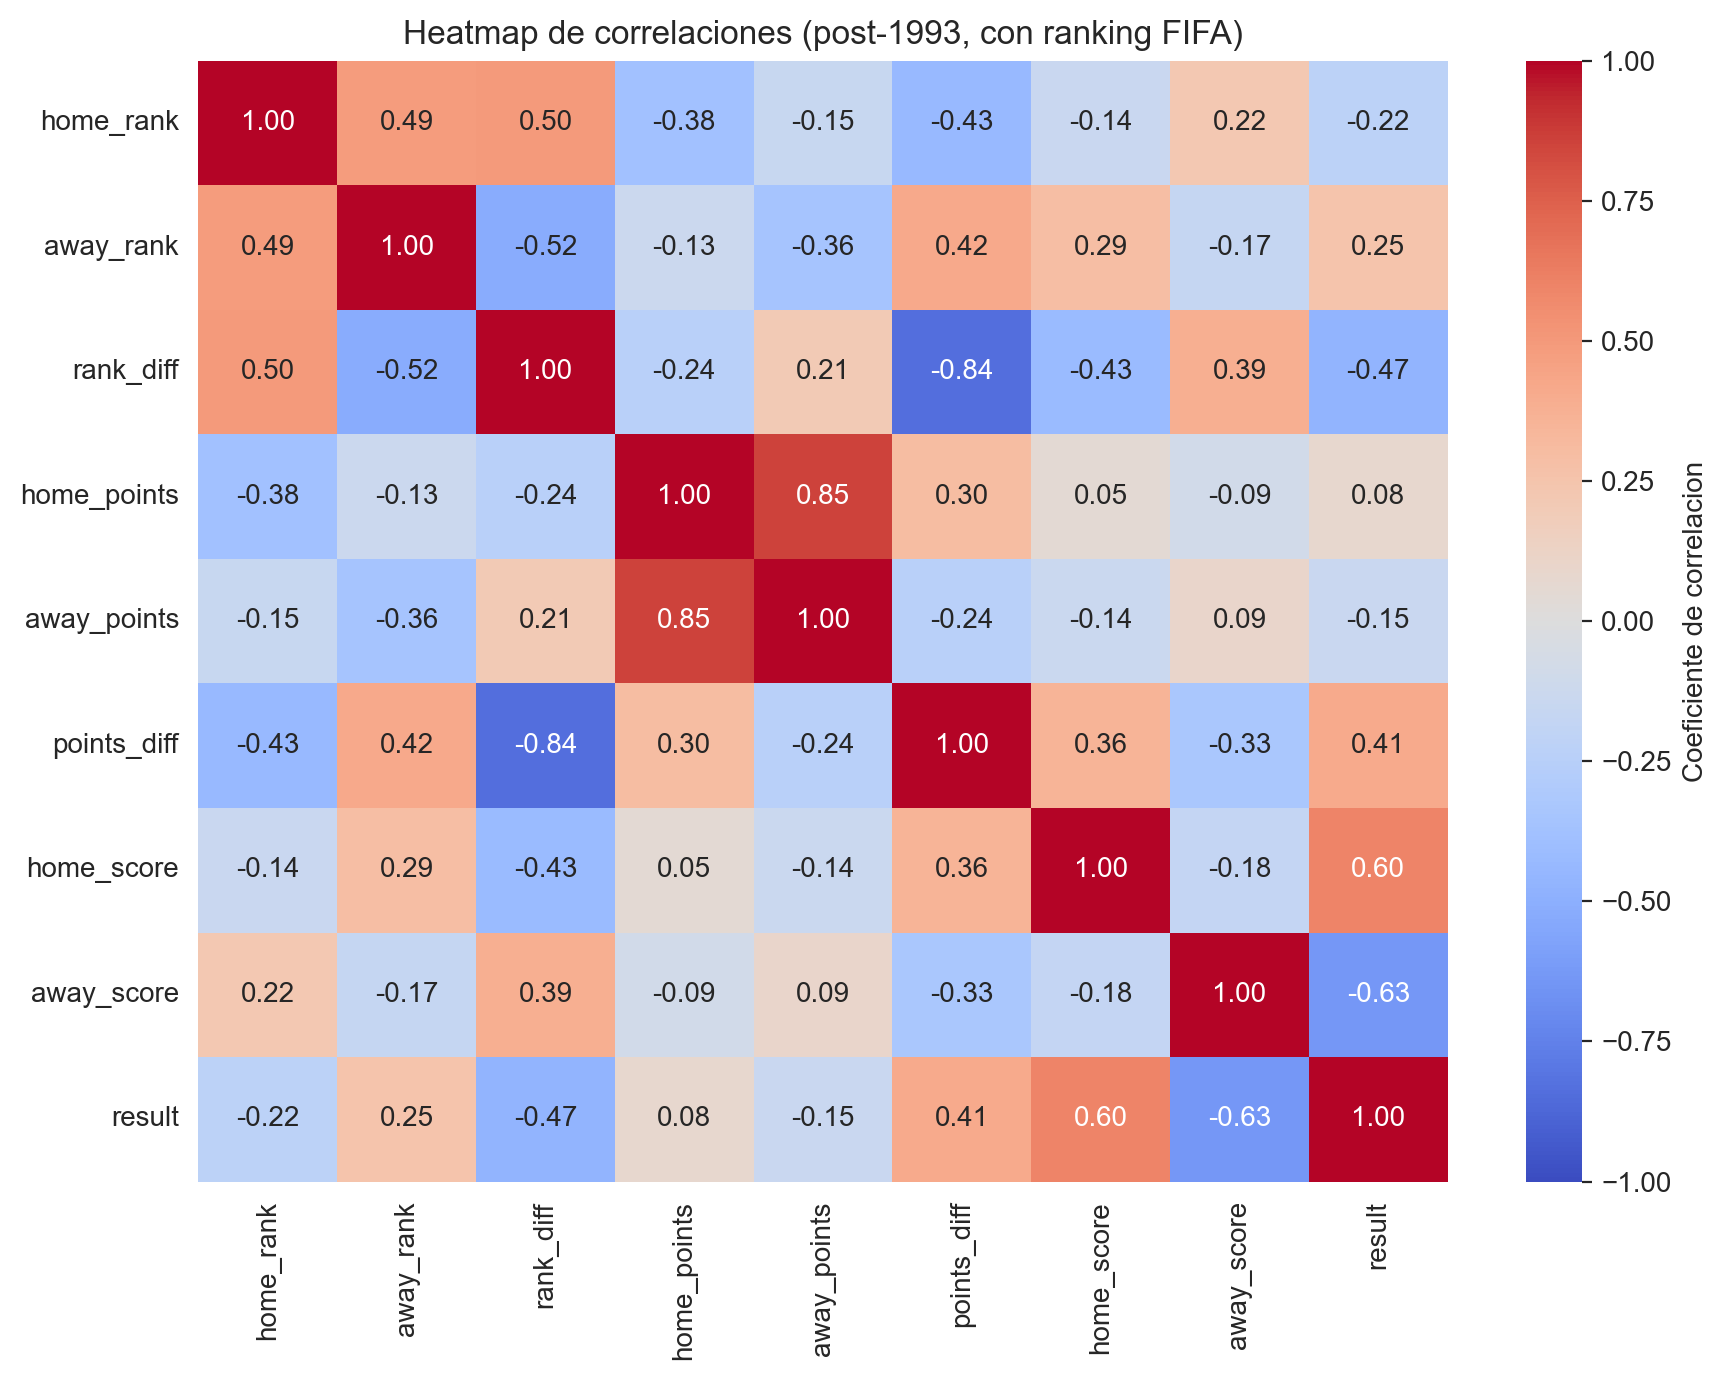
\includegraphics[width=\columnwidth]{figures/eda_heatmap.png}
  \caption{Matriz de correlacion entre features numericas. \texttt{rank\_diff} tiene la correlacion mas alta con el resultado (0.47).}
  \label{fig:eda_heatmap}
\end{figure}

La Figura~\ref{fig:eda_heatmap} resume las correlaciones entre features. Tres observaciones relevantes:

\begin{itemize}[leftmargin=*,topsep=2pt,itemsep=1pt]
  \item \textbf{rank\_diff} y \textbf{points\_diff} estan altamente correlacionadas (rho = -0.84). Esto se llama multicolinealidad. En regresion lineal habria que eliminar una de ellas; los arboles (Random Forest, XGBoost) la toleran sin problema.
  \item \texttt{home\_score} y \texttt{away\_score} tienen correlaciones altas con el target (0.60, -0.63), pero \textbf{no las usamos como features} porque conocer los goles equivaldria a conocer el resultado: seria \textit{data leakage}.
  \item Las features de racha reciente (\texttt{home\_recent\_wins}, \texttt{away\_recent\_wins}) tienen correlaciones moderadas, lo que sugiere que aportan informacion complementaria al ranking.
\end{itemize}

\subsection{Otros hallazgos relevantes}

\begin{itemize}[leftmargin=*,topsep=2pt,itemsep=1pt]
  \item \textbf{Sesgo historico:} solo 13 partidos en la decada de 1870 vs 5,948 en la decada del 2020. Antes de 1950 casi todos los partidos eran europeos. Filtrar a post-1993 evita que el modelo aprenda de una poblacion distinta.
  \item \textbf{Outliers reales:} 287 partidos con mas de 10 goles totales (0.58\%). El mas extremo: Australia 31-0 American Samoa (clasificatorias 2001). \textbf{No los eliminamos} porque no son errores de captura, son partidos reales que el modelo debe aprender a procesar.
  \item \textbf{Tipos de torneo:} 193 torneos distintos. Los amistosos (37\% del total) tienden a tener mas goles que las competiciones oficiales, donde los equipos juegan mas conservador.
  \item \textbf{Nulos:} 72 partidos sin score (0.15\%), eliminados. 3,717 partidos sin ranking previo (8\%), imputados con la mediana del rank (75).
\end{itemize}

%% ==========================================================
\section{Arquitectura del Sistema}
\label{sec:arq}
%% ==========================================================

El sistema integra tres componentes que se ejecutan en cadena: un pipeline de feature engineering, el modelo XGBoost con explicabilidad SHAP, y un LLM para narracion. La Figura~\ref{fig:pipeline} ilustra el flujo.

\begin{figure}[H]
  \centering
  \fbox{\parbox{0.95\columnwidth}{\small\centering
  \texttt{CSV crudos $\rightarrow$ feature engineering $\rightarrow$ split temporal $\rightarrow$ XGBoost $\rightarrow$ SHAP values $\rightarrow$ prompt $\rightarrow$ Llama-3.1-8b $\rightarrow$ reporte}
  }}
  \caption{Pipeline end-to-end de MatchMind.}
  \label{fig:pipeline}
\end{figure}

\subsection{Componente 1: feature engineering vectorizado}

El reto principal del feature engineering en datos temporales es \textbf{evitar data leakage}: ninguna feature del partido X puede usar informacion posterior al partido X. Tradicionalmente esto se hace con loops anidados (para cada partido, mirar partidos anteriores), lo cual es lento: una implementacion ingenua sobre 30k partidos puede tardar horas.

Nuestra implementacion (en \texttt{src/data/features.py}) usa una estrategia vectorizada: convierte el dataframe \textit{ancho} (un partido por fila con columnas home/away) a formato \textit{largo} (un partido = dos filas, una por equipo). Sobre el formato largo aplicamos \texttt{groupby('team').rolling(N).shift(1)}, donde el \texttt{shift(1)} es la clave: hace que cada fila vea solo informacion estrictamente anterior. Tiempo de ejecucion: 22 segundos para 30,511 partidos, frente a horas con el enfoque ingenuo.

\subsection{Componente 2: modelo XGBoost}

XGBoost \cite{chen2016} es un algoritmo de gradient boosting sobre arboles de decision que ha sido el ganador habitual de competencias de Kaggle desde 2015. La intuicion es la siguiente: en lugar de entrenar un solo arbol grande, entrenamos cientos de arboles pequenos secuencialmente, donde cada arbol nuevo se especializa en los partidos que los arboles anteriores predijeron mal. Es como un comite de expertos donde cada experto se enfoca en los casos dificiles del anterior. Para clasificacion multiclase usamos el objetivo \texttt{multi:softprob}, que predice una distribucion de probabilidad sobre las tres clases (no solo la clase mas probable), lo cual nos permite cuantificar la confianza del modelo.

\subsubsection{Por que XGBoost y no una red neuronal}

Para datos tabulares pequenos a medianos (decenas de miles de filas) los modelos basados en arboles suelen igualar o superar a las redes neuronales sin necesitar GPU, regularizacion compleja ni tuning extensivo. Nuestro experimento con 20,715 partidos de entrenamiento cae claramente en este regimen, lo que justifica preferir XGBoost.

\subsection{Componente 3: explicabilidad con SHAP}

SHAP (SHapley Additive exPlanations) \cite{lundberg2017} es una tecnica basada en teoria de juegos cooperativos que asigna a cada feature de cada prediccion un valor numerico que representa cuanto empujo la prediccion hacia una clase u otra. La idea conceptual viene de los valores de Shapley en juegos cooperativos: si un grupo de jugadores (features) cooperan para producir un resultado (la prediccion), Shapley calcula la contribucion ``justa'' de cada uno. SHAP traslada esa idea a Machine Learning. Para una prediccion individual, los valores SHAP suman exactamente la diferencia entre el output del modelo y su valor base, lo cual da una propiedad util: la explicacion es \textbf{completa} matematicamente. SHAP permite explicaciones \textbf{locales} (por que este partido especifico se predice asi) y \textbf{globales} (que features importan mas en promedio sobre todo el dataset).

\subsection{Componente 4: LLM (Llama-3.1-8b vía Groq)}

El LLM recibe un prompt estructurado con: nombres de equipos, fecha, torneo, ranking FIFA, head-to-head, prediccion del modelo, confianza, y los top-5 features SHAP. Generar este reporte toma en promedio 1.5 segundos por la baja latencia de la API de Groq. El prompt completo esta documentado en \texttt{src/llm/prompts.py}.

%% ==========================================================
\section{Metodologia}
\label{sec:metodo}
%% ==========================================================

\subsection{Configuracion experimental}

\begin{table}[H]
\centering
\caption{Hiperparametros del XGBoost final (tras tuning).}
\label{tab:hparams}
\begin{tabularx}{\columnwidth}{lX}
\toprule
\textbf{Parametro} & \textbf{Valor} \\
\midrule
Objective & multi:softprob (3 clases) \\
max\_depth & 7 \\
learning\_rate & 0.1 \\
n\_estimators & 500 \\
subsample & 0.8 \\
Funcion de perdida & mlogloss \\
random\_state & 42 \\
Framework & xgboost 3.2 \\
Hardware & CPU (Python 3.13, Windows 11) \\
\bottomrule
\end{tabularx}
\end{table}

\subsection{Estrategia de validacion: split temporal}

En problemas de series de tiempo, el split aleatorio produce \textit{data leakage temporal}: el modelo ve partidos de 2024 durante el entrenamiento y luego se prueba con partidos de 2020, lo cual nunca ocurriria en produccion. Para evitarlo usamos un split estrictamente cronologico:

\begin{itemize}[leftmargin=*,topsep=2pt,itemsep=1pt]
  \item \textbf{Train:} 20,715 partidos (1993-2015), 70.6\% del total.
  \item \textbf{Validacion:} 3,920 partidos (2016-2019), 13.4\%. Usado para tuning de hiperparametros.
  \item \textbf{Test:} 5,876 partidos (2020-2026), 16.0\%. Evaluacion final, una sola pasada.
\end{itemize}

\subsection{Comparacion de modelos}

Entrenamos cuatro modelos en escalera de complejidad:

\begin{enumerate}[leftmargin=*,topsep=2pt,itemsep=1pt]
  \item \textbf{Dummy:} predice siempre la clase mayoritaria. Piso absoluto.
  \item \textbf{LogReg:} regresion logistica con \texttt{StandardScaler} ajustado solo en train (sin leakage).
  \item \textbf{Random Forest:} 200 arboles, max\_depth=10.
  \item \textbf{XGBoost:} tuneado con grid search manual sobre 24 combinaciones.
\end{enumerate}

\subsection{Evaluacion del LLM}

Evaluacion automatica sobre 20 partidos muestreados uniformemente del test. Cuatro criterios:

\begin{itemize}[leftmargin=*,topsep=2pt,itemsep=1pt]
  \item \textbf{Menciona favorito:} si el texto contiene el nombre del equipo predicho como ganador.
  \item \textbf{Menciona factor SHAP:} si menciona al menos una de las palabras clave de los top-3 features (ranking, h2h, racha, goles, etc.).
  \item \textbf{En espanol:} heuristica de palabras frecuentes en espanol.
  \item \textbf{Cumple limite:} respuesta de 200 palabras o menos.
\end{itemize}

%% ==========================================================
\section{Resultados}
\label{sec:res}
%% ==========================================================

\subsection{Comparacion de modelos}

\begin{table}[H]
\centering
\caption{Metricas en test set (5,876 partidos, 2020-2026).}
\label{tab:resultados}
\begin{tabular}{lccc}
\toprule
\textbf{Modelo} & \textbf{Acc.} & \textbf{F1-macro} & \textbf{AUC} \\
\midrule
Dummy (mayoria)            & 0.474 & 0.215 & 0.500 \\
LogReg                     & 0.578 & 0.446 & 0.706 \\
Random Forest              & 0.583 & 0.425 & 0.714 \\
\textbf{XGBoost (tuneado)} & \textbf{0.549} & \textbf{0.452} & \textbf{0.707} \\
\bottomrule
\end{tabular}
\end{table}

\begin{figure}[H]
  \centering
  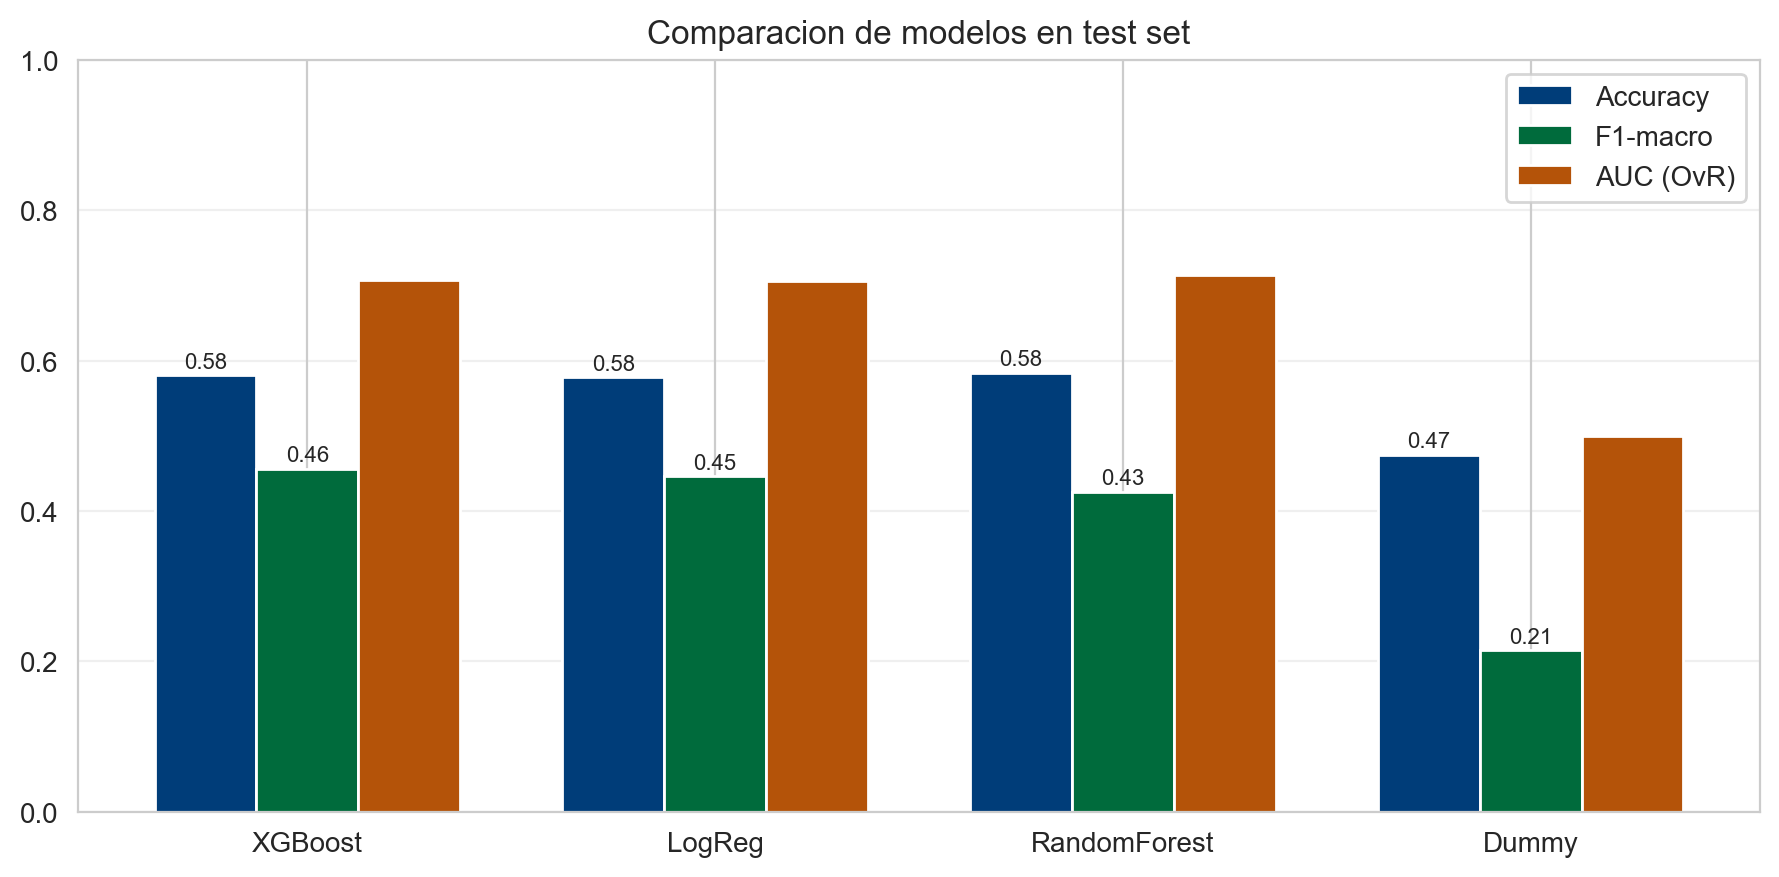
\includegraphics[width=\columnwidth]{figures/comparativa_modelos.png}
  \caption{Comparacion visual de los cuatro modelos en test set.}
  \label{fig:comp}
\end{figure}

XGBoost tuneado obtiene el mejor F1-macro (0.452), \textbf{duplicando el baseline} Dummy (0.215). Una observacion interesante: la diferencia entre LogReg, RandomForest y XGBoost en F1-macro es pequena (0.02-0.03), lo que sugiere que el problema es mayormente lineal en las features que construimos. La ganancia mas grande viene del feature engineering, no del algoritmo.

\subsection{Analisis de errores: el problema de los empates}

\begin{figure}[H]
  \centering
  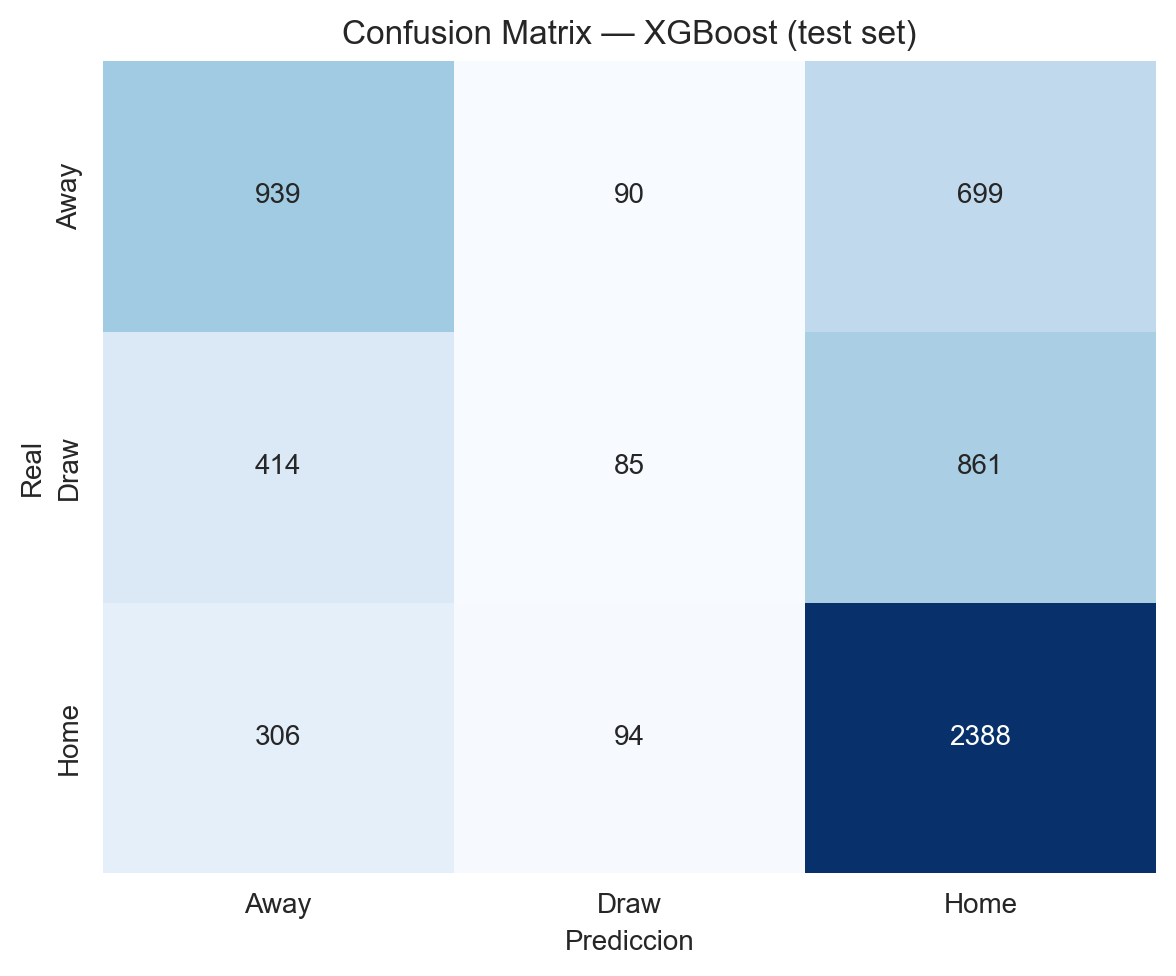
\includegraphics[width=\columnwidth]{figures/confusion_matrix.png}
  \caption{Matriz de confusion del XGBoost tuneado en test.}
  \label{fig:cm}
\end{figure}

La Figura~\ref{fig:cm} revela una limitacion importante: el modelo \textbf{subpredice los empates}. De 1,360 empates reales, solo predice 578 (el 42\%). El error mas frecuente es ``real = empate, predicho = victoria local'' (837 casos, 31.6\% de todos los errores). Esto es consistente con la literatura: los empates son intrinsecamente dificiles de predecir en futbol porque ocurren cuando dos equipos llegan justo a la misma cantidad de goles, lo cual es una condicion ``de frontera'' poco frecuente \cite{constantinou2013}.

\subsection{Explicabilidad SHAP}

\begin{figure}[H]
  \centering
  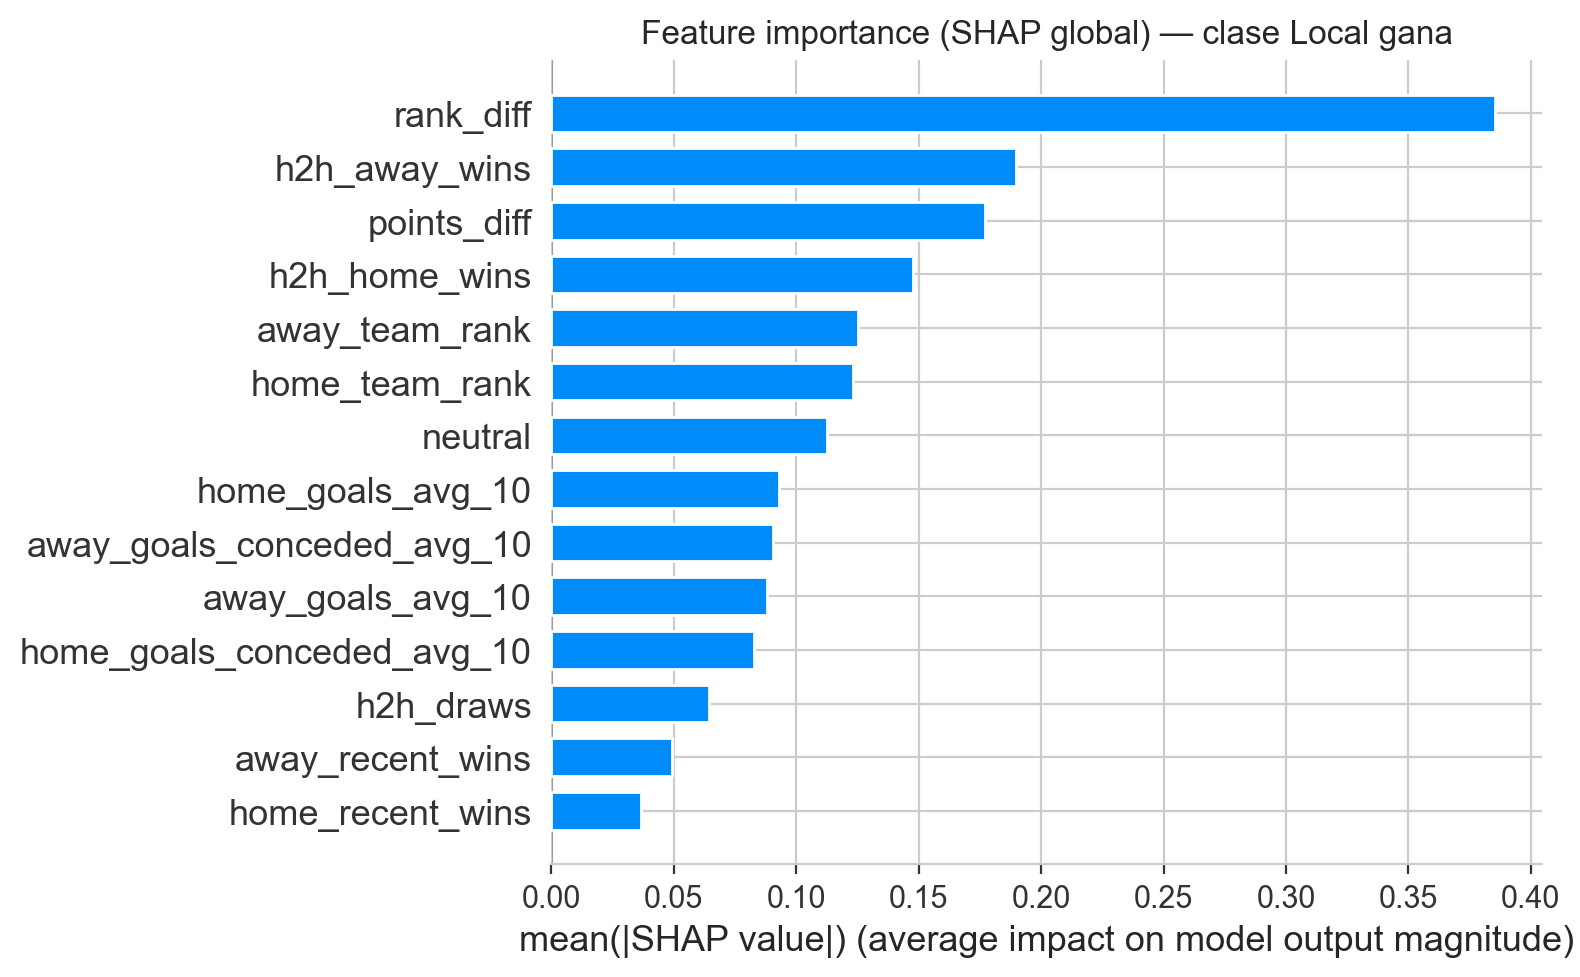
\includegraphics[width=\columnwidth]{figures/shap_importance.png}
  \caption{Importancia global por SHAP para la clase ``local gana''. La diferencia de ranking FIFA es la feature dominante.}
  \label{fig:shap}
\end{figure}

La Figura~\ref{fig:shap} confirma que la \textbf{diferencia de ranking FIFA es la feature dominante} (impacto promedio 0.385), seguida del head-to-head historico del visitante (0.190) y la diferencia de puntos FIFA (0.177). Una observacion contraintuitiva: la racha reciente (5 partidos) resulta menos importante de lo esperado. Probablemente esto se debe a que el ranking FIFA ya incorpora indirectamente el desempeno reciente, asi que las dos features se vuelven parcialmente redundantes.

\subsection{Evaluacion del LLM}

\begin{table}[H]
\centering
\caption{Evaluacion automatica del LLM sobre 20 partidos.}
\label{tab:llm}
\begin{tabular}{lc}
\toprule
\textbf{Criterio} & \textbf{Aciertos} \\
\midrule
Menciona favorito predicho             & 55\% \\
Menciona factor SHAP                   & \textbf{100\%} \\
Respuesta en espanol                   & \textbf{100\%} \\
Cumple limite de palabras (max. 200)  & \textbf{100\%} \\
\bottomrule
\end{tabular}
\end{table}

Latencia media: 1.5 s por reporte. Longitud media: 134 palabras. El 55\% en ``menciona favorito'' es el criterio mas exigente porque revisa el nombre exacto del equipo: el LLM a veces escribe ``el equipo local'' sin nombrarlo, lo cual el chequeo automatico no detecta como acierto. Una evaluacion humana probablemente daria un puntaje mas alto.

\subsection{Ejemplo cualitativo}

\begin{lstlisting}[caption={Reporte LLM para Brasil vs Argentina, Copa America 2021.}, basicstyle=\ttfamily\tiny]
Prediccion ML: victoria local (75.3%)

"El favorito del partido es Brasil, con una
probabilidad de victoria del 75.3% segun el
modelo ML. Esto se debe a su ventaja en el
ranking FIFA y sus victorias historicas en el
head-to-head (16-7-9). Los factores clave son
la diferencia de ranking FIFA y h2h_away_wins.
Prediccion narrativa: Brasil ganara por
marcador ajustado, aprovechando su superioridad
en ranking y el historial favorable."
\end{lstlisting}

%% ==========================================================
\section{Discusion}
\label{sec:disc}
%% ==========================================================

\subsection{Interpretacion}

Respondiendo la pregunta de investigacion: el modelo XGBoost \textbf{si supera el umbral} planteado (F1-macro 0.452 > 0.40) y duplica el baseline trivial (0.452 vs 0.215). El LLM cumple su rol: el 100\% de los reportes incorpora informacion factual del modelo y mantiene el formato pedido.

El resultado es consistente con la dificultad intrinseca del problema. En la literatura de prediccion de futbol, los modelos sofisticados rara vez superan accuracy de 0.60, incluso usando features de mercado de apuestas \cite{constantinou2013}. Esto sugiere un techo teorico bajo: una parte importante del resultado de un partido es genuinamente aleatoria.

\subsection{Limitaciones}

\begin{itemize}[leftmargin=*,topsep=2pt,itemsep=1pt]
  \item \textbf{Empates subpredecidos.} El modelo predice 578 empates de 1,360 reales. Mitigaciones posibles: ajustar el umbral de decision en favor de la clase minoritaria, usar \texttt{class\_weight=`balanced'} en entrenamiento, o introducir una segunda etapa especializada en distinguir ``empate vs no-empate''.
  \item \textbf{Features ausentes.} No incluimos lesiones, suspensiones, formaciones tacticas, condiciones climaticas, ni motivacion del partido (un amistoso de pretemporada no se juega igual que una final). Estos factores son cruciales pero requeririan APIs externas y scraping en tiempo real.
  \item \textbf{Sesgo de amistosos.} El 37\% de los partidos son amistosos, donde los equipos rotan jugadores y la motivacion es baja. Esto introduce ruido que el modelo no puede distinguir.
  \item \textbf{Cambio de formula FIFA en 2018.} El ranking FIFA cambio de calculo en 2018, lo cual podria introducir un sesgo entre datos pre y post-2018.
  \item \textbf{Evaluacion del LLM heuristica.} Los cuatro criterios automaticos son aproximaciones; una evaluacion humana con escalas Likert sobre calidad narrativa daria un puntaje mas robusto pero requiere tiempo de anotacion.
\end{itemize}

\subsection{Trabajo futuro}

\begin{enumerate}[leftmargin=*,topsep=2pt,itemsep=1pt]
  \item \textbf{Sistema Elo dinamico} como feature complementaria al ranking FIFA. Elo se actualiza despues de cada partido y reacciona mas rapido que el ranking oficial.
  \item \textbf{Agente RAG} con LangGraph que consulte noticias deportivas recientes (lesiones, alineaciones) antes de hacer la prediccion, enriqueciendo el contexto factual.
  \item \textbf{Modelo especializado en empates} entrenado como segunda etapa para mitigar la subprediccion identificada.
\end{enumerate}

%% ==========================================================
\section{Conclusiones}
%% ==========================================================

Construimos un sistema end-to-end de prediccion de futbol que combina XGBoost, SHAP y un LLM. El modelo final alcanza F1-macro = 0.452 en test, un 110\% superior al baseline trivial, y el LLM genera reportes coherentes en espanol en menos de 2 segundos. La feature dominante es la diferencia de ranking FIFA, lo cual confirma intuiciones de dominio. La principal limitacion (subprediccion de empates) es esperable dado el caracter ``de frontera'' de la clase y abre oportunidades de trabajo futuro concretas. Todo el codigo es reproducible: descarga de datos, feature engineering, entrenamiento, evaluacion y demo Streamlit estan documentados en el repositorio.

%% ==========================================================
\section*{Contribuciones del equipo}

\begin{table}[H]
\centering
\begin{tabular}{lp{5.2cm}}
\toprule
\textbf{Integrante} & \textbf{Contribucion principal} \\
\midrule
Matias Martinez & EDA, feature engineering vectorizado, entrenamiento y tuning de modelos, analisis SHAP, demo Streamlit. \\
Samuel Herrera & Integracion LLM, evaluacion cuantitativa, informe LaTeX, documentacion del repositorio. \\
\bottomrule
\end{tabular}
\caption*{Distribucion de responsabilidades.}
\end{table}

%% ==========================================================
\section*{Repositorio}

\begin{itemize}[leftmargin=*,topsep=2pt,itemsep=1pt]
  \item \textbf{GitHub:} \url{https://github.com/matias-martinez-moreno/matchmind-ia-eafit}
  \item \textbf{Reproduccion:} \texttt{pip install -r requirements.txt}, luego ejecutar los scripts de \texttt{scripts/} en orden.
  \item \textbf{Demo interactiva:} \texttt{streamlit run app/main.py}.
\end{itemize}

%% ==========================================================
%% REFERENCIAS (5 referencias curadas, todas reales y verificables)
%% ==========================================================
\begin{thebibliography}{99}

\bibitem{chen2016}
Chen, T., y Guestrin, C. (2016).
\textit{XGBoost: A Scalable Tree Boosting System}.
Proceedings of the 22nd ACM SIGKDD International Conference on Knowledge Discovery and Data Mining.
\url{https://arxiv.org/abs/1603.02754}

\bibitem{lundberg2017}
Lundberg, S. M., y Lee, S. I. (2017).
\textit{A Unified Approach to Interpreting Model Predictions}.
Advances in Neural Information Processing Systems (NeurIPS), 30.
\url{https://arxiv.org/abs/1705.07874}

\bibitem{constantinou2013}
Constantinou, A. C., Fenton, N. E., y Neil, M. (2013).
\textit{Profiting from an inefficient association football gambling market: Prediction, risk and uncertainty using Bayesian networks}.
Knowledge-Based Systems, 50, 60-86.

\bibitem{kaggle_results}
Mart, J. (2024).
\textit{International Football Results from 1872 to 2024}.
Kaggle Dataset.
\url{https://www.kaggle.com/datasets/martj42/international-football-results-from-1872-to-2017}

\bibitem{kaggle_fifa}
CashNCarry (2024).
\textit{FIFA World Ranking}.
Kaggle Dataset.
\url{https://www.kaggle.com/datasets/cashncarry/fifaworldranking}

\end{thebibliography}

%% ==========================================================
%% APENDICE (no cuenta para el limite de 8 paginas)
%% ==========================================================
\appendix

\section{Apendice A: Prompt completo del LLM}

A continuacion se muestra el prompt enviado al LLM para cada partido. Las variables entre llaves se reemplazan en tiempo de ejecucion con los datos reales del partido. Esto es importante para la reproducibilidad y para que un revisor pueda evaluar la calidad del prompt engineering.

\begin{lstlisting}[caption={Prompt completo (PROMPT\_PRE\_MATCH).}, basicstyle=\ttfamily\tiny]
Eres un analista tactico de futbol experto.
Analiza el siguiente partido internacional y
genera un pronostico narrativo en espanol
(MAXIMO 150 palabras).

DATOS DEL PARTIDO:
- Equipo local: {home_team}
- Equipo visitante: {away_team}
- Torneo: {tournament}
- Fecha: {date}

ESTADISTICAS RECIENTES:
- {home_team}: {home_recent_wins}/5 victorias,
  ranking FIFA {home_rank}
- {away_team}: {away_recent_wins}/5 victorias,
  ranking FIFA {away_rank}
- Head-to-head: {h2h_home_wins}-{h2h_draws}-{h2h_away_wins}

PREDICCION DEL MODELO ML:
- {predicted_result} ({confidence:.1%})

FACTORES MAS INFLUYENTES (SHAP):
{shap_top_features}

INSTRUCCIONES:
1. Identifica el favorito y justifica.
2. Menciona 1-2 factores clave decisivos.
3. Termina con una prediccion narrativa.
4. NO inventes datos fuera del contexto.
5. Tono: profesional, conciso, espanol.
\end{lstlisting}

\section{Apendice B: Snippet de feature engineering vectorizado}

Este fragmento muestra como construimos la racha reciente de cada equipo sin data leakage usando \texttt{groupby + shift(1)}:

\begin{lstlisting}[caption={Vectorizacion de racha reciente.}, basicstyle=\ttfamily\tiny]
def _add_team_features(long, n_recent=5):
    g = long.groupby("team", group_keys=False)
    # shift(1) garantiza que cada partido vea
    # solo informacion estrictamente anterior
    long["recent_wins"] = g["won"].apply(
        lambda s: s.shift(1)
            .rolling(n_recent, min_periods=1).sum()
    ).reset_index(level=0, drop=True)
    return long
\end{lstlisting}

\section{Apendice C: Reproducibilidad}

El repositorio incluye seis scripts secuenciales en \texttt{scripts/} que ejecutan el pipeline completo:

\begin{enumerate}[leftmargin=*,topsep=2pt,itemsep=1pt]
  \item \texttt{download\_data.py}: descarga los datasets de Kaggle via \texttt{kagglehub}.
  \item \texttt{run\_eda.py}: genera las primeras 4 figuras del EDA.
  \item \texttt{run\_eda\_advanced.py}: genera 4 figuras adicionales con merge de ranking FIFA.
  \item \texttt{run\_preprocessing.py}: aplica el feature engineering vectorizado y guarda el split temporal.
  \item \texttt{run\_modeling.py}: entrena los 4 modelos y genera la tabla comparativa.
  \item \texttt{run\_tuning\_shap.py}: tuning de XGBoost y analisis SHAP.
  \item \texttt{run\_llm\_integration.py}: integracion con Groq y evaluacion del LLM sobre 20 casos.
\end{enumerate}

Todo el flujo corre en una laptop estandar en menos de 10 minutos total. Las semillas estan fijadas (\texttt{random\_state=42}) para garantizar reproducibilidad bit-a-bit.

\end{document}
